\documentclass[letterpaper,12pt,twoside=false,DIV=11]{scrartcl}

%----------------------CONFIG---------------------------
%math packages
\usepackage{amsmath,amssymb,amsthm,units,unitsdef}

%bibliography style and citation style, bibstyles to use: plainnat, abbrvnat, unsrtnat, named, chicago
%otherwise numerical citationstyle will be used
%\usepackage[authoryear,round]{natbib}

\usepackage{longtable,tabularx,tabulary,multirow,lscape}
\usepackage[font={sl},format=plain,labelfont=bf]{caption}

% colors
\usepackage{color,colortbl}
\usepackage[dvipsnames]{xcolor}
\definecolor{darkblue}{HTML}{00354C}

\usepackage{booktabs}
%\usepackage{showkeys} % shows the labels above the references for

%easier development
\usepackage{ifpdf}

\ifpdf
    \usepackage[pdftex]{graphicx}
    \usepackage[]{pdfpages} %for including full pdf pages
    \usepackage[pdftex,
        bookmarks,
        bookmarksopen=true,
        bookmarksnumbered=true,
        pdfauthor={Reto Trappitsch},
        pdftitle={On the origin of elements in the Milky Way - Homework},
        colorlinks,
        linkcolor=darkblue,
        citecolor=darkblue,
        filecolor=black,
        urlcolor=darkblue,
        anchorcolor=black,
        menucolor=black,
        breaklinks=true,
        pageanchor=true, %for jumping to a page
        plainpages=false,
        pdfpagelabels=true]{hyperref}
    \pdfcompresslevel=9
    \pdfoutput=1
    \DeclareGraphicsExtensions{.pdf,.png,.jpg,.jpeg}
\else
    \usepackage{graphicx}
\fi
\usepackage{rotating} % rotate figures
\usepackage{subcaption}
\usepackage{wrapfig}


\usepackage{fancyhdr}
\pagestyle{fancy}
%\addtolength{\headwidth}{\marginparsep} %these change header-rule width
%\addtolength{\headwidth}{\marginparwidth}
\lhead{}
\chead{\small\scshape On the Origin of Elements in the Milky Way} 
\rhead{} 
\lfoot{} 
\cfoot{\thepage} 
\rfoot{} 
\renewcommand{\headrulewidth}{.3pt} 
\renewcommand{\footrulewidth}{.3pt}

% Redefine author as topic
\newcommand{\topic}{\author}

%
%Redefining sections as problems
%
\makeatletter
\newenvironment{problem}{\@startsection
    {section}
    {1}
    {-.2em}
    {-3.5ex plus -1ex minus -.2ex}
    {2.3ex plus .2ex}
    {
        \pagebreak[3] % forces pagebreak when space is small; use \eject for better results
        \noindent\sffamily\bfseries Problem
    }
}
{
    %\vspace{1ex}\begin{center} \rule{0.3\linewidth}{.3pt}\end{center}}
    \begin{center}\large\bfseries\ldots\ldots\ldots\end{center}
}
\makeatother

% set enumerate to use letters
\renewcommand{\theenumi}{\alph{enumi}}

% newcommands
%============
% my short cuts
\providecommand{\e}[1]{\ensuremath{\times 10^{#1}}}
\providecommand{\ex}[1]{\ensuremath{^{#1}}}
\providecommand{\dex}[1]{\ensuremath{\delta^{#1}}}
\newcommand{\nean}{$^{22}$Ne($\alpha$,n)$^{25}$Mg}

% textnormal
\newcommand{\tn}{\textnormal}
% textregistered
\newcommand{\tr}{$^\tn{\textregistered}$}


%-------------------DOCUMENT---------------------------

\begin{document}


\title{Homework \#3 -- Solution}
\topic{The Sun}

\maketitle
\thispagestyle{fancy}
\begin{problem}{The Salpeter process (20\%)}
\begin{enumerate}
    \item{Including the $3\alpha$ process results in the following figure:\\ \\
    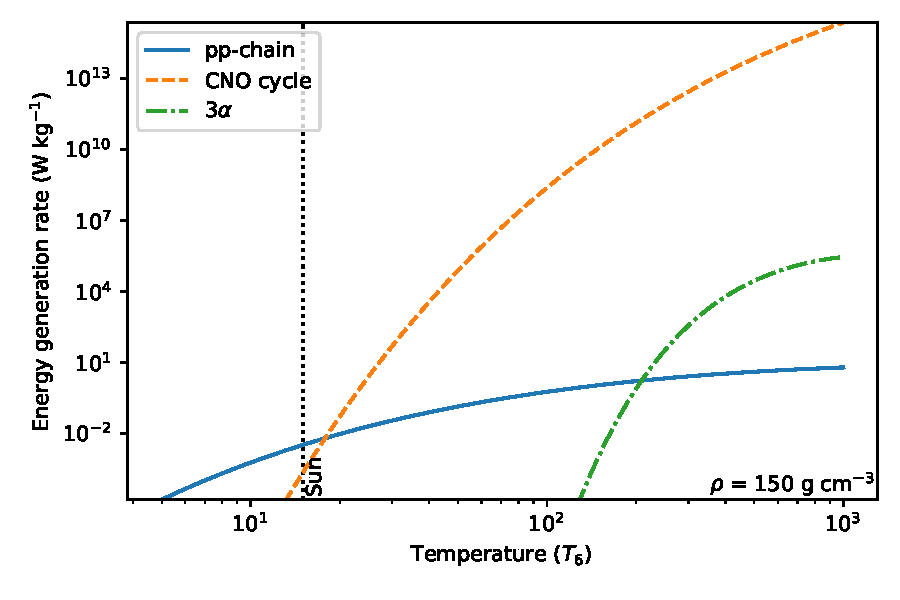
\includegraphics[width=0.75\textwidth]{energy_generation_sun}}
    \item The temperature in the center of the Sun is roughly 15\,MK. This is far too low to turn on the $3\alpha$-process, see above Figure. 
    \item An electric field can, in the presence of free charge carriers, be dampened. This is the so-called screening effect. In the plasma at the center of the Sun, the electrons are free charge carriers. They partially shield the $\alpha$-nuclei from each other, thus screening the Coulomb barrier that exists between them. This enhances the $3\alpha$ process. See also \href{https://en.wikipedia.org/wiki/Electric-field_screening}{Wikipedia}.
\end{enumerate}
\end{problem}

\begin{problem}{Why do we have carbon (20\%)}
The $3\alpha$ reaction is highly enhanced thanks to a resonance in the \ex{12}C molecule, which effectively boosts this otherwise improbable reaction rate. This resonance was predicted in 1954 by Fred Hoyle and is thus today known as the Hoyle state.
\end{problem}

\begin{problem}{Fate of the Earth (20\%)}
During the AGB phase, the Sun will expand so massivly that its radius will reach out to around the orbit of Earth. From the Hertzsprung-Russle Diagram in Figure 4.6 we can see that the approximate surface temperature of the Sun will be around $3000\,$K. The Earth will thus get at least that hot during the death of the Sun.
\end{problem}

\begin{problem}{Helix nebula (20\%)}
\begin{enumerate}
    \item{Below figure shows a sketch of the situation:\\ \\
          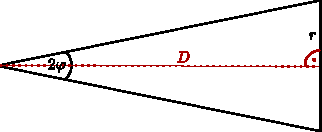
\includegraphics[width=0.5\textwidth]{helix_nebula_sketch}\\
          Here, $2\phi = 16'$ is the diameter of the nebula, $D = 213$\, the distance, and $r$ the radius of the nebula. The diameter of the nebula can then be calculated as:
          \begin{align}
              \frac{r}{d} &= \tan(\varphi)\\
              r &= d \tan(\varphi) = 0.5\,\mathrm{pc} 
          \end{align}}
          The nebula thus has a diameter of around 1\,pc.
    \item Assuming the nebla expanded from a point outwards, the distance it has moved up to today at a velocity of $v=20$\,km\,s$^{-1}$ is $r$. The age of the nebula can thus be calculated as
    \begin{equation}
        t = \frac{r}{v} = 24\,\mathrm{ka}.
    \end{equation}
\end{enumerate}

\end{problem}

\begin{problem}{Population II stars (20\%)}
\begin{enumerate}
    \item If these stars formed 1\,Ga after the Big Bang, they would today be roughly 13\,Ga old. Using equation~(4.28) we can calculate the minimum mass that such a star would have, assuming it is about to die right now. This mass is then
    \begin{equation}
        M = M_\odot \left(\frac{10\,\mathrm{Ga}}{14\,\mathrm{Ga}}\right)^{1/2.5} = 0.87\,M_\odot.
    \end{equation}
    \item These stars are fairly difficult to observe because they have a mass that is lower than the solar mass. Using equation (4.27) we can estimate their luminosity to be at most $0.6L_\odot$. This makes these stars faint and thus powerful telescopes are required in order to observe them.
\end{enumerate}
\end{problem}

\end{document}
